\section{Introduction}
Innodisk cloud administration platform (iCAP) is a remote device management system for both private and public clouds, which primarily focuses on storage device management and monitoring.
This document will describe the iCAP client service application programming interface (API), which be a bridge from the external sensors or remote devices to the iCAP client service.

\subsection{Client Service API Overview}
In this section, we will take a brief introduce for the iCAP client service API.
The iCAP client service API was implemented with GNU-C programming language, which is a popular programming language nowadays.

The iCAP client service API architecture are shown as figure~\ref{fig:apiarch}:
	\begin{figure}[H]
		\centering
		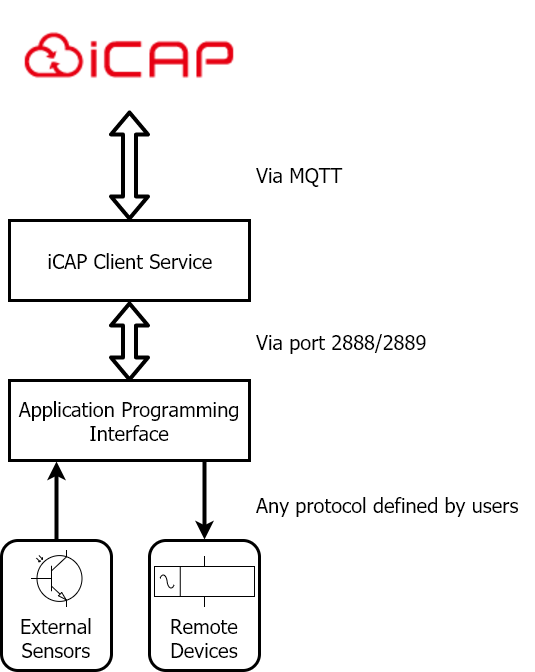
\includegraphics[width=10cm]{pic/apiarch}
		\caption{iCAP client service API architecture \label{fig:apiarch}}
	\end{figure}
While the iCAP client service was working, it will upload the data which collected from the devices in each interval defined by users.
The default of client service collection data are including:
\begin{itemize}
	\item Operating system information
	\item CPU information
	\item Motherboard information
	\item Memory information
	\item Storage information
	\item Networking information
\end{itemize}

When users wants to add its own external sensor, just using the API register into the iCAP client service.
However, users need to provide the identity name, type, unit, and the callback function for this sensor.
The iCAP client service will collect the external sensor data via the callback function which was registered before uploading the raw data.
The remote device are using similar technique to connection with iCAP client service, the difference is the callback function are triggered only on the client service receive the remote commands.

\subsection{API architecute}
The iCAP client service API file architecture is shown as following:
\setlength{\DTbaselineskip}{20pt}
\DTsetlength{1em}{3em}{0.5em}{2pt}{4pt}
\dirtree{%
	.1 /iCAP client servce API.
		.2 /windows.
			.3 /include.
				.4 libiCAPClient.h.
			.3 libiCAPClient.dll.
			.3 libjson-c-2.dll.
		.2 /linux.
			.3 /include.
				.4 libiCAPClient.h.
			.3 libiCAPClient\_32.a.
			.3 libiCAPClient\_64.a.
}
Since the iCAP client service API using the json format to encode/decode the packages, the only dependence library is {\em json-c}.
The following command is a reference for install json-c library on Ubuntu:
\begin{lstlisting}[language=bash,frame=single]
$ sudo apt-get install libjson0 libjson0-dev
\end{lstlisting}
However, the library was including in the same package while on Windows.

\subsection{Reference Material}
Here we list some reference link about the dependence libraries:
\begin{itemize}
	\item JSON-C: https://github.com/json-c/json-c/wiki
\end{itemize}